\documentclass{beamer}
\usetheme{default}

\title{Viva La Libertad carajo!}
\author{Emmanuel Arias}
\begin{document}
\begin{frame}[plain]
    \maketitle
\end{frame}

\begin{frame}
  \centering
  Las opiniones y perspectivas expresadas en esta presentación son exclusivamente mías y no representan, en forma alguna, las posturas oficiales de la organización de esta conferencia, de mi empleador, ni de ninguna otra entidad o afiliación a la que esté vinculado. Esta exposición busca fomentar el análisis crítico y el diálogo, y no debe interpretarse como una promoción o respaldo de ninguna posición institucional.
\end{frame}

\begin{frame}{¿Libertad, hay una sola?}
  \begin{minipage}{0.45\textwidth}
        \centering
        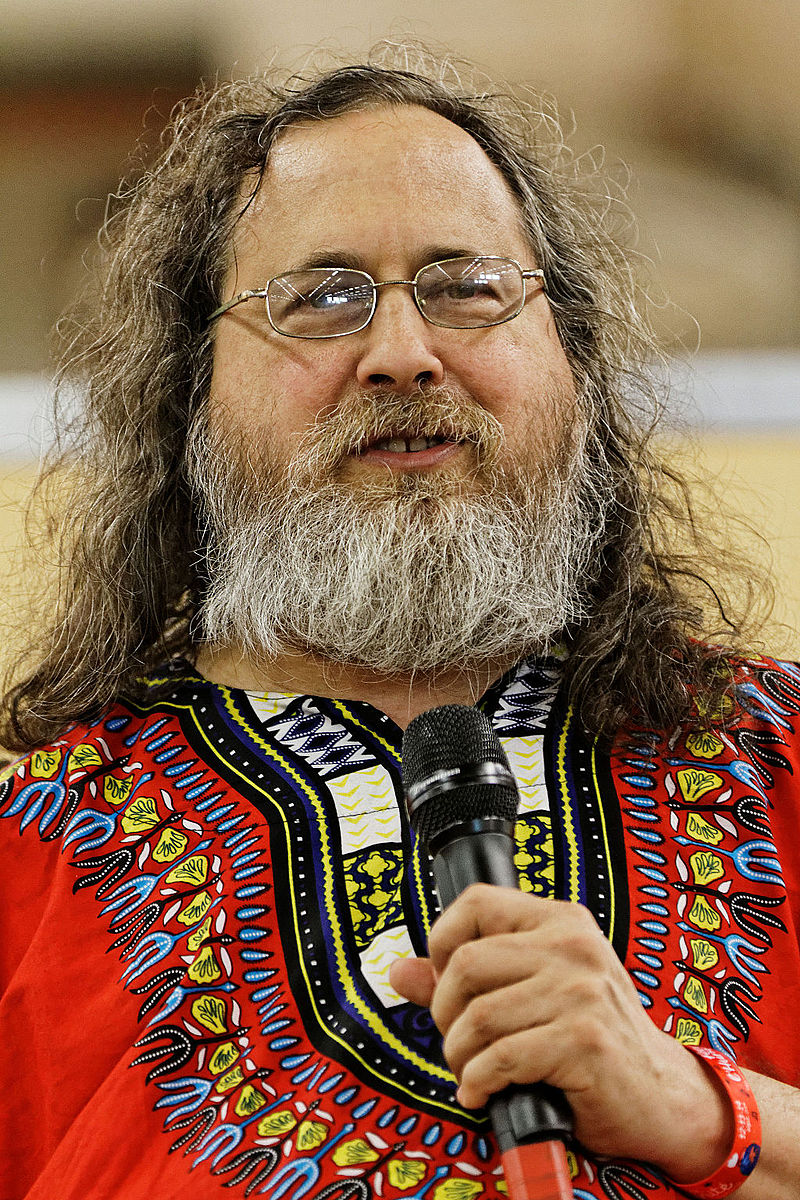
\includegraphics[width=\linewidth]{images/rms.jpg}
        \captionof{figure}{Richard Stallman}
    \end{minipage}
    \hfill
    \begin{minipage}{0.45\textwidth}
        \centering
        
\includegraphics[width=\linewidth]{images/milei.jpg}
        \captionof{figure}{Javier Milei}
    \end{minipage}
\end{frame}

\begin{frame}{La libertad de Richard Stallman}
  \begin{itemize}
  \item Para Stallman, la libertad es la capacidad de controlar la tecnología que utilizamos. Es un concepto ético y moral, no solo técnico. \pause
  \item El software libre es cuestión de libertad, no de precio. Para entender el concepto, debes pensar en libertad como en 'libertad de expresión', no como en 'cerveza gratis'.
\end{frame}

\begin{frame}
    \centering
    \Huge ¿Qué es la libertad?
\end{frame}
\end{document}
